\chapter{Proposta}
\label{sec:Proposal}

Aproveitando os princípios do método IVF apresentados na Seção~\ref{sec:ivf}, como manipulação genética e melhoramento seletivo, é possível explorar formas de melhorar a convergência e a diversidade das soluções geradas~\cite{camilo-junior2011}. O uso desses recursos pode resultar em soluções de maior qualidade que capturam melhor os compromissos entre diferentes objetivos em problemas de otimização multi-objetivo.

Os parâmetros do IVF, como a Taxa de Execução~``$r$'' e o Tamanho da Coleta~``$c$'', governam o equilíbrio entre a geração de novos indivíduos e a intensidade das manipulações genéticas internas. Ambos são projetados para serem controlados pelo operador com base nas necessidades ou características específicas do problema. Estudos e experimentações anteriores sugerem valores padrão para esses parâmetros. Por exemplo, uma Taxa de Execução~``$r$'' é frequentemente definida em torno de 10\% com base em trabalhos fundamentais do IVF~\cite{sampaio2017ivf, sampaio2019ivf}. A calibração de~``$r$'' é particularmente crucial, pois define a frequência de intervenção do IVF. Essa modulação cuidadosa da influência do módulo é essencial para garantir que ele contribua positivamente para o processo de otimização, apoiando, em vez de interromper, a evolução da população principal na busca por soluções ótimas.

Similarmente, o Tamanho da Coleta~``$c$'', que dita a quantidade de material genético coletado que entra no processo de melhoramento seletivo do módulo, também frequentemente assume um valor padrão em torno de 10\% do tamanho da população principal, com base em evidências empíricas de estudos anteriores~\cite{sampaio2017ivf, sampaio2019ivf}. Este padrão sugerido para~``$c$'' visa encontrar um equilíbrio eficaz entre o aprimoramento da qualidade da solução e o gerenciamento do consumo de avaliações de função. Isso ocorre porque a magnitude de~``$c$'' impacta diretamente a carga computacional; um tamanho de coleta maior leva a um número maior de avaliações realizadas pelo algoritmo IVF auxiliar. De fato, empregar um~``$c$'' excessivamente grande pode ser contraproducente devido ao consumo elevado de avaliações, uma preocupação observada em trabalhos derivados que exploram a integração do IVF com outros algoritmos como NSGA-II e GDE3~\cite{sampaio2017ivf, sampaio2019ivf}. Portanto, embora um~``$c$'' maior implique que mais material genético é processado e potencialmente soluções mais diversas são geradas durante a execução do módulo, é imperativo considerar cuidadosamente seu impacto substancial no orçamento geral de avaliações.

Ao selecionar e alternar os valores dessas variáveis, podemos explorar diferentes formas de realizar a manipulação genética e adaptá-las de acordo com os requisitos e características específicas da otimização do problema tratado. Essa flexibilidade permite uma exploração abrangente de várias técnicas de manipulação genética dentro do método IVF, aumentando sua eficácia e adaptabilidade na resolução de problemas de otimização multi-objetivo. Reconhecendo os benefícios da hibridização de algoritmos evolutivos e observando diferentes características e um compromisso entre intensificação e exploração na versão canônica do SPEA2, vale a pena investigar o acoplamento do método IVF com o algoritmo SPEA2, que já alcança resultados superiores em alguns problemas em comparação com outros algoritmos evolutivos multi-objetivo~\cite{zitzler2000comparison,zitzler2001spea2}.

Portanto, a proposta deste trabalho, denominada IVF/SPEA2, preserva a integridade do fluxo operacional padrão do SPEA2, conforme delineado na literatura~\cite{zitzler2001spea2}. No entanto, um mecanismo de acoplamento integrativo~\cite{blum2011hybrid} é integrado no ponto de geração de novas soluções, como pode ser visto na Figura~\ref{fig:ivf_spea2_flow}. Dentro desta estrutura, a execução do método IVF em qualquer geração é contingente ao total de Avaliações de Função (FEs) consumidas até o momento. Consequentemente, o processo pelo qual o algoritmo hospedeiro (SPEA2) gera novos indivíduos deve ser adaptado para operar dentro de um orçamento predefinido ($N$) de FEs atribuído por geração.

\begin{figure*}[htbp]
\centering
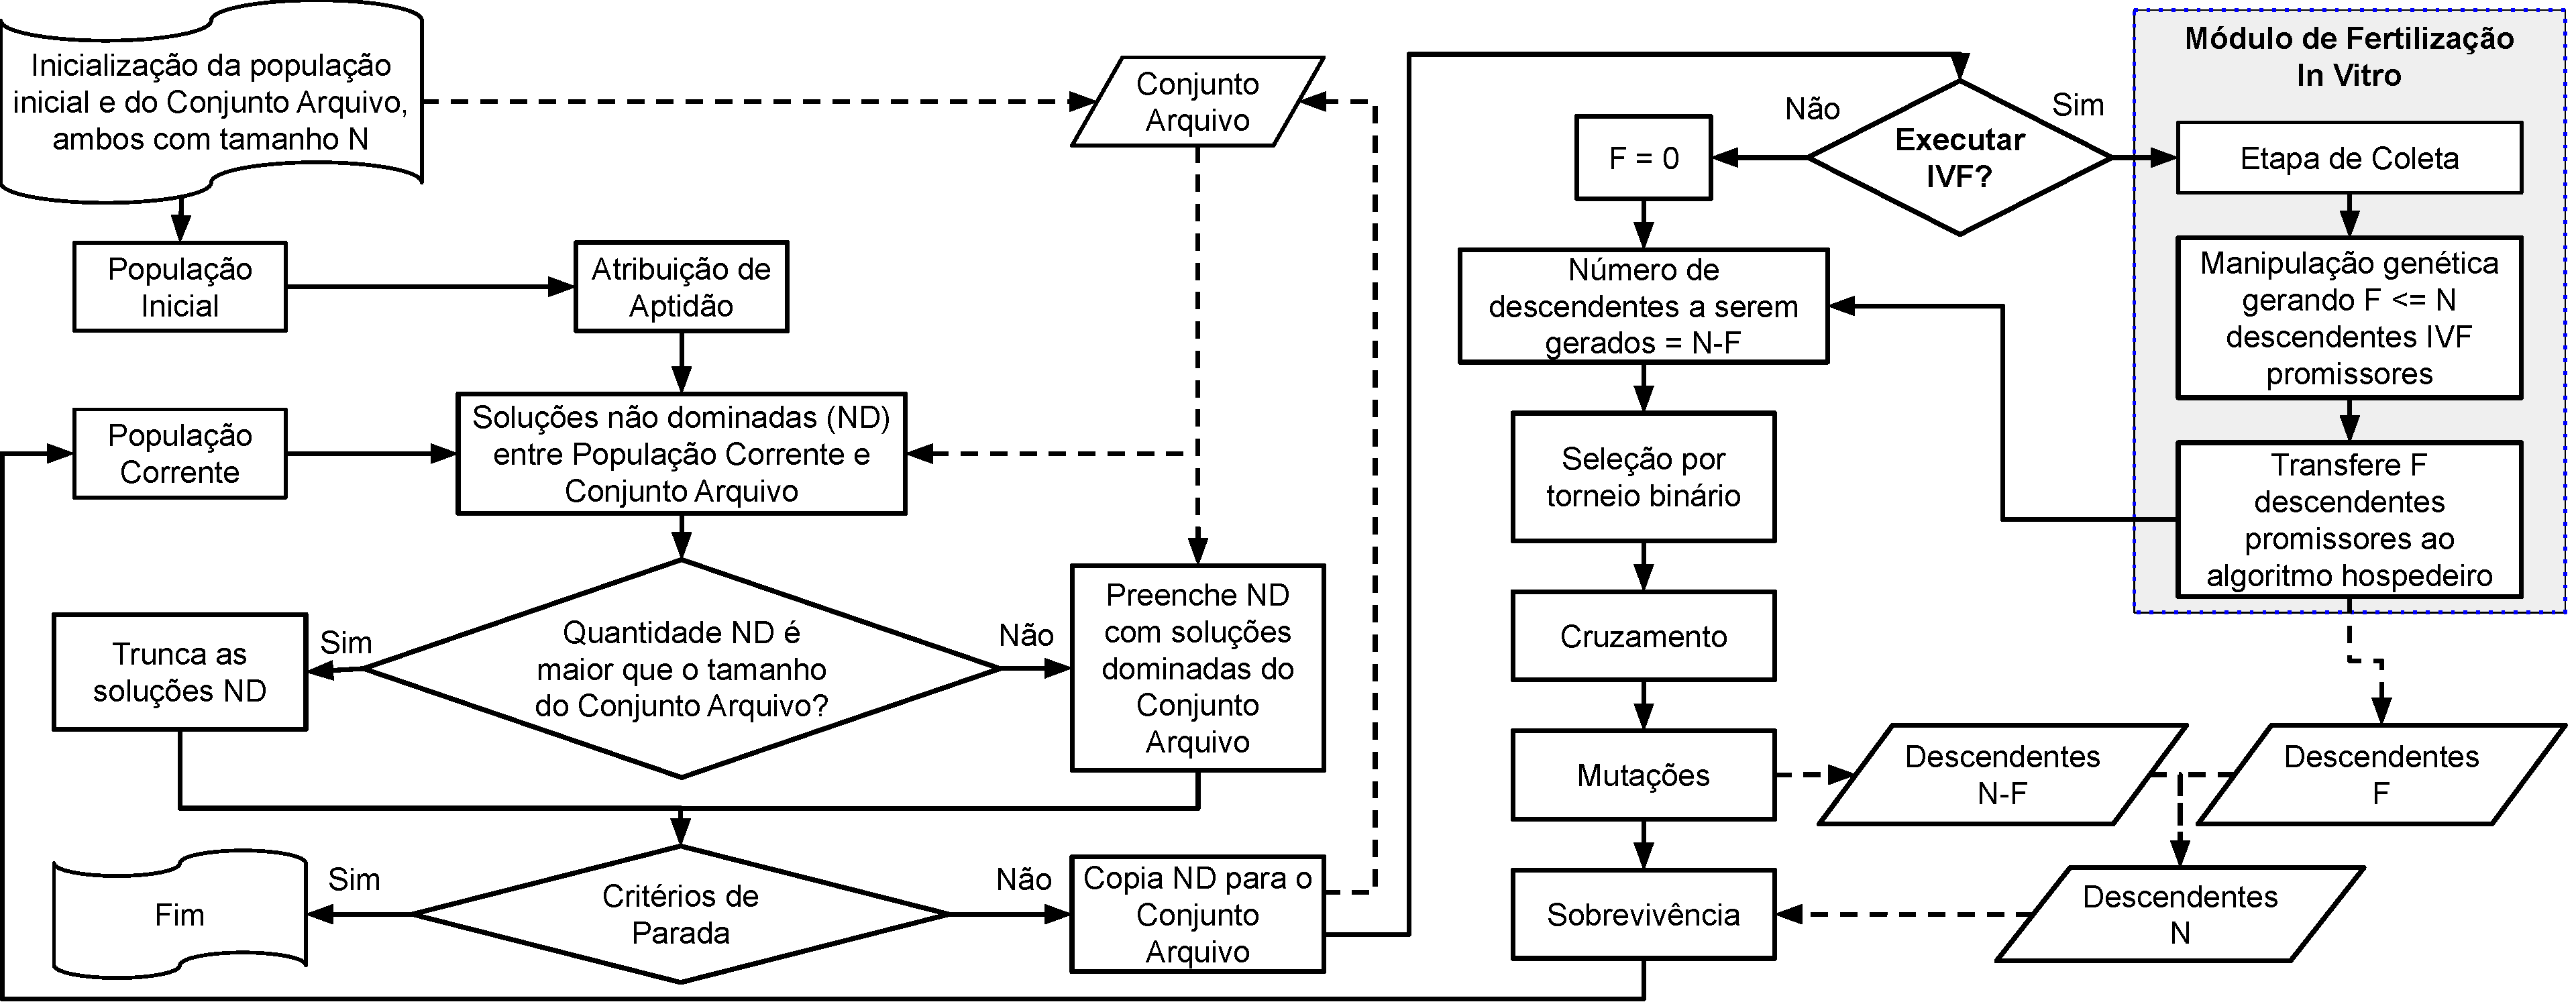
\includegraphics[width=\textwidth]{fig/fluxo_ivfspea2_pt.pdf}
\caption{O fluxo do algoritmo IVF/SPEA2. \textbf{Legenda:} Linhas contínuas representam o fluxo principal do algoritmo hospedeiro SPEA2; linhas tracejadas indicam fluxo condicional e integração do módulo IVF; a caixa com cor diferente destaca o Módulo de Fertilização \textit{In Vitro} como um componente adicional; setas bidirecionais mostram a troca de informações entre o algoritmo hospedeiro e o módulo IVF; nós de decisão (losangos) representam pontos de controle para as decisões do algoritmo.}
\label{fig:ivf_spea2_flow}
\end{figure*}

Na Figura~\ref{fig:ivf_spea2_flow}, pode-se observar o diagrama de fluxo de trabalho do algoritmo híbrido proposto (IVF/SPEA2). Seguindo os passos do algoritmo SPEA2, as operações básicas são fundamentadas da mesma forma, aderindo à filosofia evolutiva e elitista proposta por Zitzler et al.~\cite{zitzler2001spea2}. Visando a evolução e o equilíbrio entre diversificação e convergência, introduzimos o método IVF logo antes de gerar os descendentes tradicionais no fluxo hospedeiro, permitindo-nos gerar descendentes em número igual ao de indivíduos na população ao final de uma geração.

\section{Adaptações para a Integração com o SPEA2}

O principal diferencial do IVF/SPEA2 em comparação com acoplamentos anteriores (IVF/NSGA-II e IVF/GDE3) reside na adaptação da estratégia de comparação para determinar ciclos sucessivos no módulo IVF. No IVF/NSGA-II e IVF/GDE3, a comparação baseava-se na relação de dominância direta entre o indivíduo gerado e a(s) solução(ões) de elite atual(is), usando a dominância de Pareto para determinar se um novo ciclo deveria ser iniciado.

No entanto, considerando a estratégia específica do SPEA2, onde a melhor aptidão (menor valor numérico, já que $F(i)$ é minimizado conforme a Equação~\ref{eq:final_fitness}) nem sempre representa o indivíduo mais adequado na população uma vez que o $k$-ésimo vizinho mais próximo (onde $k = \lfloor\sqrt{N + \overline{N}}\rfloor$, conforme definido na Seção~\ref{sec:spea2}) é considerado ao calcular distâncias para outras soluções na estimativa de densidade (Equação~\ref{eq:density_estimation}), enquanto o NSGA-II examina o vizinho mais próximo usando a distância de aglomeração (\textit{crowding distance}) decidimos adaptar a abordagem para examinar se um novo indivíduo gerado no fluxo estava entre os $2 \times c$ indíviduos com menor valor para $F(i)$. Aqui, ``$c$'' representa o parâmetro de tamanho da coleta, e toda a população conhecida consiste em $N + \overline{N}$ indivíduos, onde $N$ é o tamanho da população principal e $\overline{N}$ é o tamanho do Conjunto Arquivo (ambos iguais a $N$ no SPEA2).

Essa modificação foi necessária devido à abordagem diferenciada do SPEA2 para o tratamento da densidade populacional em comparação com outros MOEAs. Enquanto o NSGA-II usa a distância de aglomeração considerando apenas o vizinho mais próximo para cálculos de densidade, o SPEA2 usa o $k$-ésimo vizinho mais próximo, onde a densidade é calculada como descrito na Equação~\ref{eq:density_estimation}. No SPEA2, a melhor aptidão (valor numericamente menor de $F(i)$) nem sempre indica o indivíduo mais adequado para seleção, pois considera a distribuição espacial das soluções no espaço objetivo, ao contrário do NSGA-II, onde uma melhor aptidão (baseada no \textit{ranking} de dominância e na distância de aglomeração) geralmente indica maior qualidade da solução.

A verificação da aptidão determina se a solução gerada está entre as $2 \times c$ melhores soluções (aquelas com os menores valores de $F(i)$) de acordo com a função de aptidão do SPEA2 (Equação~\ref{eq:final_fitness}), onde $R(i)$ é a aptidão bruta baseada na força de dominância (Equação~\ref{eq:raw_fitness}), e $D(i)$ é a estimativa de densidade (Equação~\ref{eq:density_estimation}). Se essa condição for atendida, um novo ciclo se inicia, usando a solução derivada com a melhor aptidão (menor valor de $F(i)$) como doadora primária para operações subsequentes. Essa adaptação permite que o IVF/SPEA2 aproveite totalmente a lógica de aptidão do SPEA2, mantenha a consistência com a filosofia de seleção baseada em densidade do algoritmo hospedeiro e preserve as características específicas de diversidade e convergência do SPEA2.

\section{Estágios do Módulo IVF}

O método IVF opera através de quatro estágios distintos, cada um com papéis específicos no processo de otimização híbrida, conforme ilustrado na Figura~\ref{fig:ivf_spea2_flow}:

\subsection{Gatilho de Ativação}

O gatilho de ativação determina quando o módulo IVF deve ser executado durante o processo evolutivo. Este mecanismo é baseado no parâmetro~``$r$'', que representa a porcentagem do total de avaliações que o IVF consumirá. O gatilho é ativado de acordo com o número de Avaliações de Função (FE) utilizadas até o momento atual, permitindo que o fluxo permaneça inalterado por algumas gerações, mantendo o comportamento do SPEA2 canônico. Isso fornece controle refinado sobre a frequência da interferência do IVF, evitando o descarrilamento da evolução da população e permitindo a calibração da influência do IVF no processo global de otimização.

\subsection{Estágio de Coleta}

O estágio de coleta reúne material genético de alta qualidade da população atual para manipulação. Este processo envolve a seleção de soluções promissoras com base na aptidão do SPEA2 e é controlado pelo parâmetro~``$c$''(tamanho da coleta). Um valor maior de ``$c$'' resulta em mais avaliações realizadas e uma maior quantidade de material genético disponível para manipulação genética. O critério de seleção utiliza a função de aptidão do SPEA2 $F(i) = R(i) + D(i)$ (Equação~\ref{eq:final_fitness}), considerando tanto a dominância ($R(i)$) quanto a densidade ($D(i)$), garantindo a representatividade e a qualidade das soluções coletadas para o processo de fertilização \textit{in vitro}.

\subsection{Manipulação Genética}

O estágio de manipulação genética realiza operações genéticas especializadas no material coletado para gerar novos indivíduos promissores. As estratégias disponíveis incluem os diferentes operadores de recombinação descritos na Seção~\ref{sec:ivf}: modificações sutis em soluções conhecidas para intensificação (AR), geração de soluções completamente novas para diversificação (EAR-N), e alternância entre estratégias de acordo com as características do problema (EAR-T, EAR-P, EAR-PA). Essa flexibilidade permite a exploração abrangente de diferentes técnicas de manipulação genética, adaptação a necessidades específicas do problema e configurações personalizáveis de compromisso entre intensificação e exploração. O controle de qualidade limita a geração a $F \leq N$ indivíduos por ciclo, com múltiplos ciclos possíveis até que todas as avaliações alocadas sejam consumidas.

\subsection{Estágio de Transferência}

O estágio de transferência integra soluções superiores geradas pelo IVF ao algoritmo hospedeiro. O critério de transferência requer que as soluções estejam entre os $2 \times c$ melhores indivíduos (aqueles com os menores valores de $F(i)$) da população completa ($N + \overline{N}$ indivíduos), avaliadas com base na função de aptidão do SPEA2, garantindo que apenas material genético de alta qualidade seja transferido. O processo de integração transfere $F$ soluções superiores para o algoritmo hospedeiro enquanto ajusta o número de descendentes tradicionais para $N-F$, mantendo o tamanho da população consistente ($N$ indivíduos). Se uma solução derivada classificar-se entre as melhores, um novo ciclo é iniciado usando a solução derivada com a melhor aptidão (menor valor de $F(i)$) como doadora primária, permitindo potencialmente a transcendência de barreiras anteriormente intransponíveis na busca pela fronteira de Pareto ótima.

O método IVF opera com o parâmetro~``$r$'' que representa a porcentagem do total de avaliações que ele consumirá, permitindo que o fluxo permaneça inalterado por algumas gerações, como no SPEA2 canônico. Quando o método IVF é ativado e conclui sua execução, existe o potencial para que soluções promissoras derivadas de outras soluções de qualidade sejam integradas ao algoritmo hospedeiro (etapa de transferência), permitindo a transcendência de barreiras anteriormente intransponíveis e avançando ainda mais em direção à fronteira ótima de Pareto.

Dentro deste processo, múltiplos ciclos podem ocorrer, consumindo potencialmente todas as avaliações alocadas para a geração. Um novo ciclo se inicia quando uma solução derivada de soluções promissoras se classifica entre as melhores soluções da população. A comparação é baseada na aptidão da população conforme a função $F(i) = R(i) + D(i)$ do SPEA2, e é aqui que entra uma das principais adaptações projetadas para se alinhar melhor com a lógica de consideração de aptidão do SPEA2.

Através das diversas estratégias de manipulação genética do IVF, o elitismo pode ser aumentado ou reduzido ao longo das gerações, fazendo pequenas modificações em soluções coletadas conhecidas ou gerando soluções inteiramente novas. Isso cria novas configurações de compromisso  entre diversificação e intensificação, seguindo os princípios de hibridização de algoritmos evolutivos apresentados na Seção~\ref{sec:hibridizacao}. A abordagem visa facilitar a adaptação das configurações de intensificação e diversificação para otimizar domínios de problemas específicos, aproveitando as características complementares do SPEA2 e do método IVF.